\chapter{Labeling und Datensätze}\label{ch:labeling-und-datensatze}

Für die Evaluation der Klassifikation ist es nötig, zuvor entsprechende Testdatensätze mit Annotationen bereitzustellen. Ein solcher Datensatz besteht dabei aus mehreren Testfällen, wobei jeder Testfall ein \ac{BPMN}-Prozessmodell darstellt. Standardisierte Datensätze gewährleisten einheitliche Prüfbedingungen und ermöglichen so objektive Leistungsvergleiche.

\section{Labeling Tool}\label{sec:labeling-tool}

Um die Erstellung und Verwaltung von gelabelten \ac{BPMN}-Prozessmodellen zu erleichtern, wurde eine Webapp entwickelt. Mit dieser können \ac{BPMN}-Testfälle erstellt, bearbeitet und Aktivitäten mit Labeln versehen werden. Wichtige Funktionen des Labeling-Tools sind dabei: (1) das Anlegen und Verwalten von Datensätzen, (2) die Erstellung beliebig vieler Testfälle pro Datensatz, (3) die direkte Bearbeitung von \ac{BPMN}-Modellen im Browser mittels BPMN.io \cite{bpmnio}, (4) ein Labeling-Modus, in dem Aktivitäten als \ac{DSGVO}-kritisch markiert und optional mit einer Begründung versehen werden können, sowie (5) die persistente Speicherung der annotierten Testfälle in einer Datenbank zur späteren Nutzung im Evaluationsframework (siehe Kapitel~\ref{ch:evaluationsframework}).

Abbildung \ref{fig:labeling-editor} zeigt den Labeling-Editor im Labeling-Modus. Die in der Abbildung nummerierten Bereiche strukturieren die Oberfläche und das Zusammenspiel der Funktionen:

\begin{figure}[h]
    \centering
    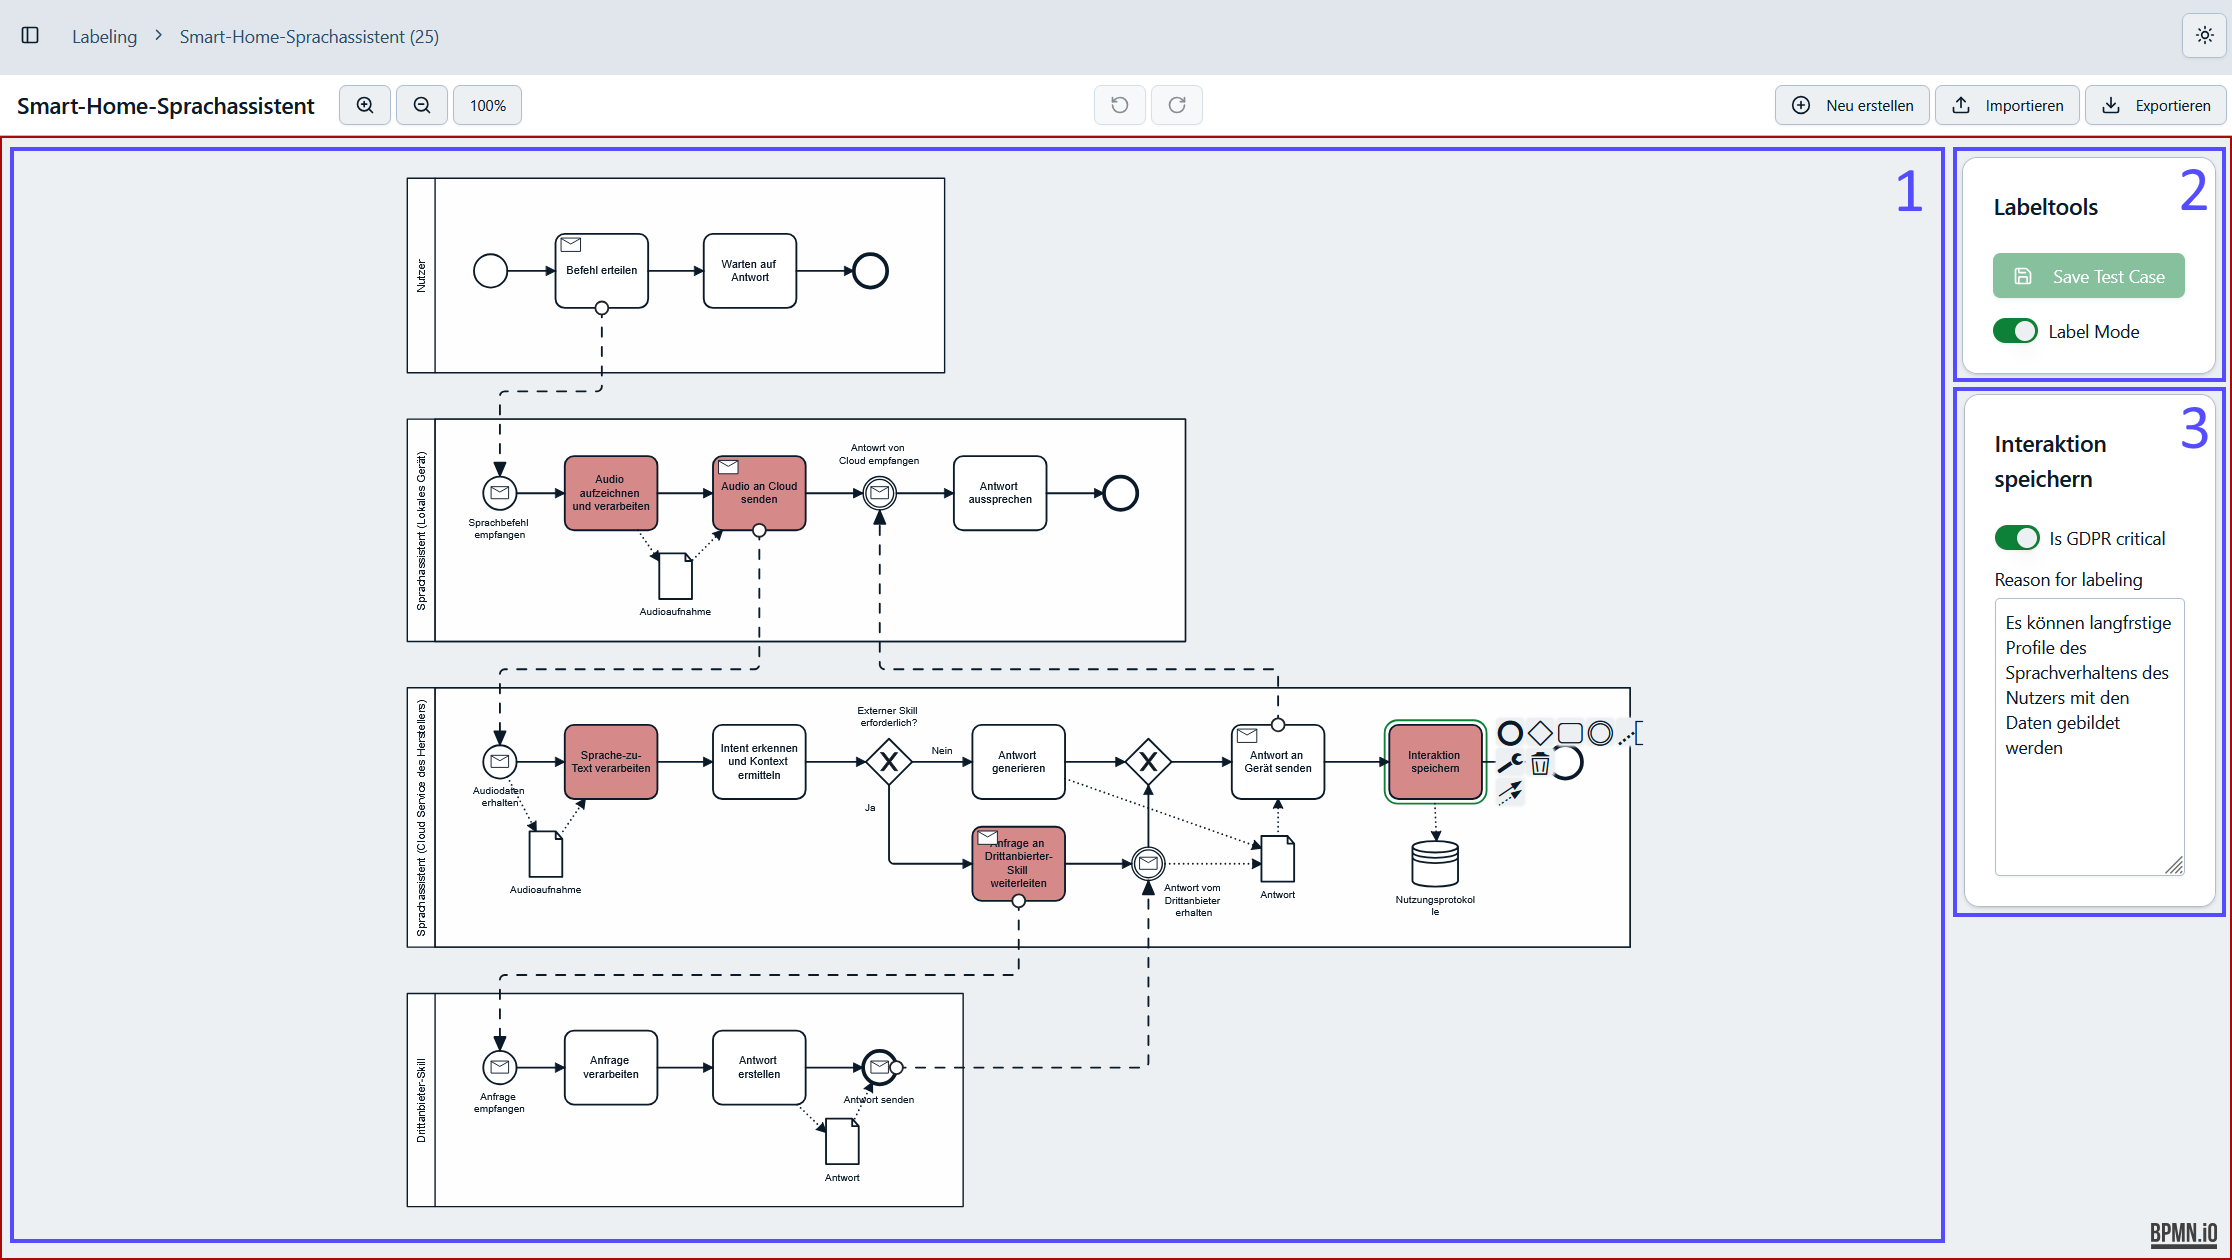
\includegraphics[width=\textwidth]{images/labeling/labeling-editor-annotated}
    \caption{Labeling-Editor im Labeling-Modus mit exemplarischem Modell.}
    \label{fig:labeling-editor}
\end{figure}

\begin{enumerate}
    \item \textbf{BPMN-Editor} (linke Hauptfläche): Hier werden Prozessmodelle erstellt, importiert, bearbeitet und angezeigt. Im Labeling-Modus ist die Modellierung bewusst gesperrt. Die Elemente können dann nur ausgewählt werden, um sie zu labeln. Als kritisch gelabelte Aktivitäten werden im Modell farblich hervorgehoben und sind damit sofort visuell erkennbar.
    \item \textbf{Label-Tools} (rechte Seitenleiste oben): Über dieses Panel wird zwischen Editier- und Labeling-Modus gewechselt und ein Testfall gespeichert.
    \item \textbf{Label-Panel der Aktivität} (rechte Seitenleiste unten): Ist eine Aktivität ausgewählt, kann sie hier als \enquote{DSGVO-kritisch} markiert werden. Zusätzlich lässt sich optional eine natürlichsprachige Begründung hinterlegen. Diese Begründung dient ausschließlich der Dokumentation und Nachvollziehbarkeit und wird nicht in der Evaluierung berücksichtigt.
\end{enumerate}

In der Übersicht der Datensätze aus Abbildung \ref{fig:labeling-datasets} sind alle angelegten Datensätze und zugehörigen Testfälle aufgelistet. Von hier aus können neue Datensätze und Testfälle erstellt sowie bestehende bearbeitet werden.

\begin{figure}[h]
    \centering
    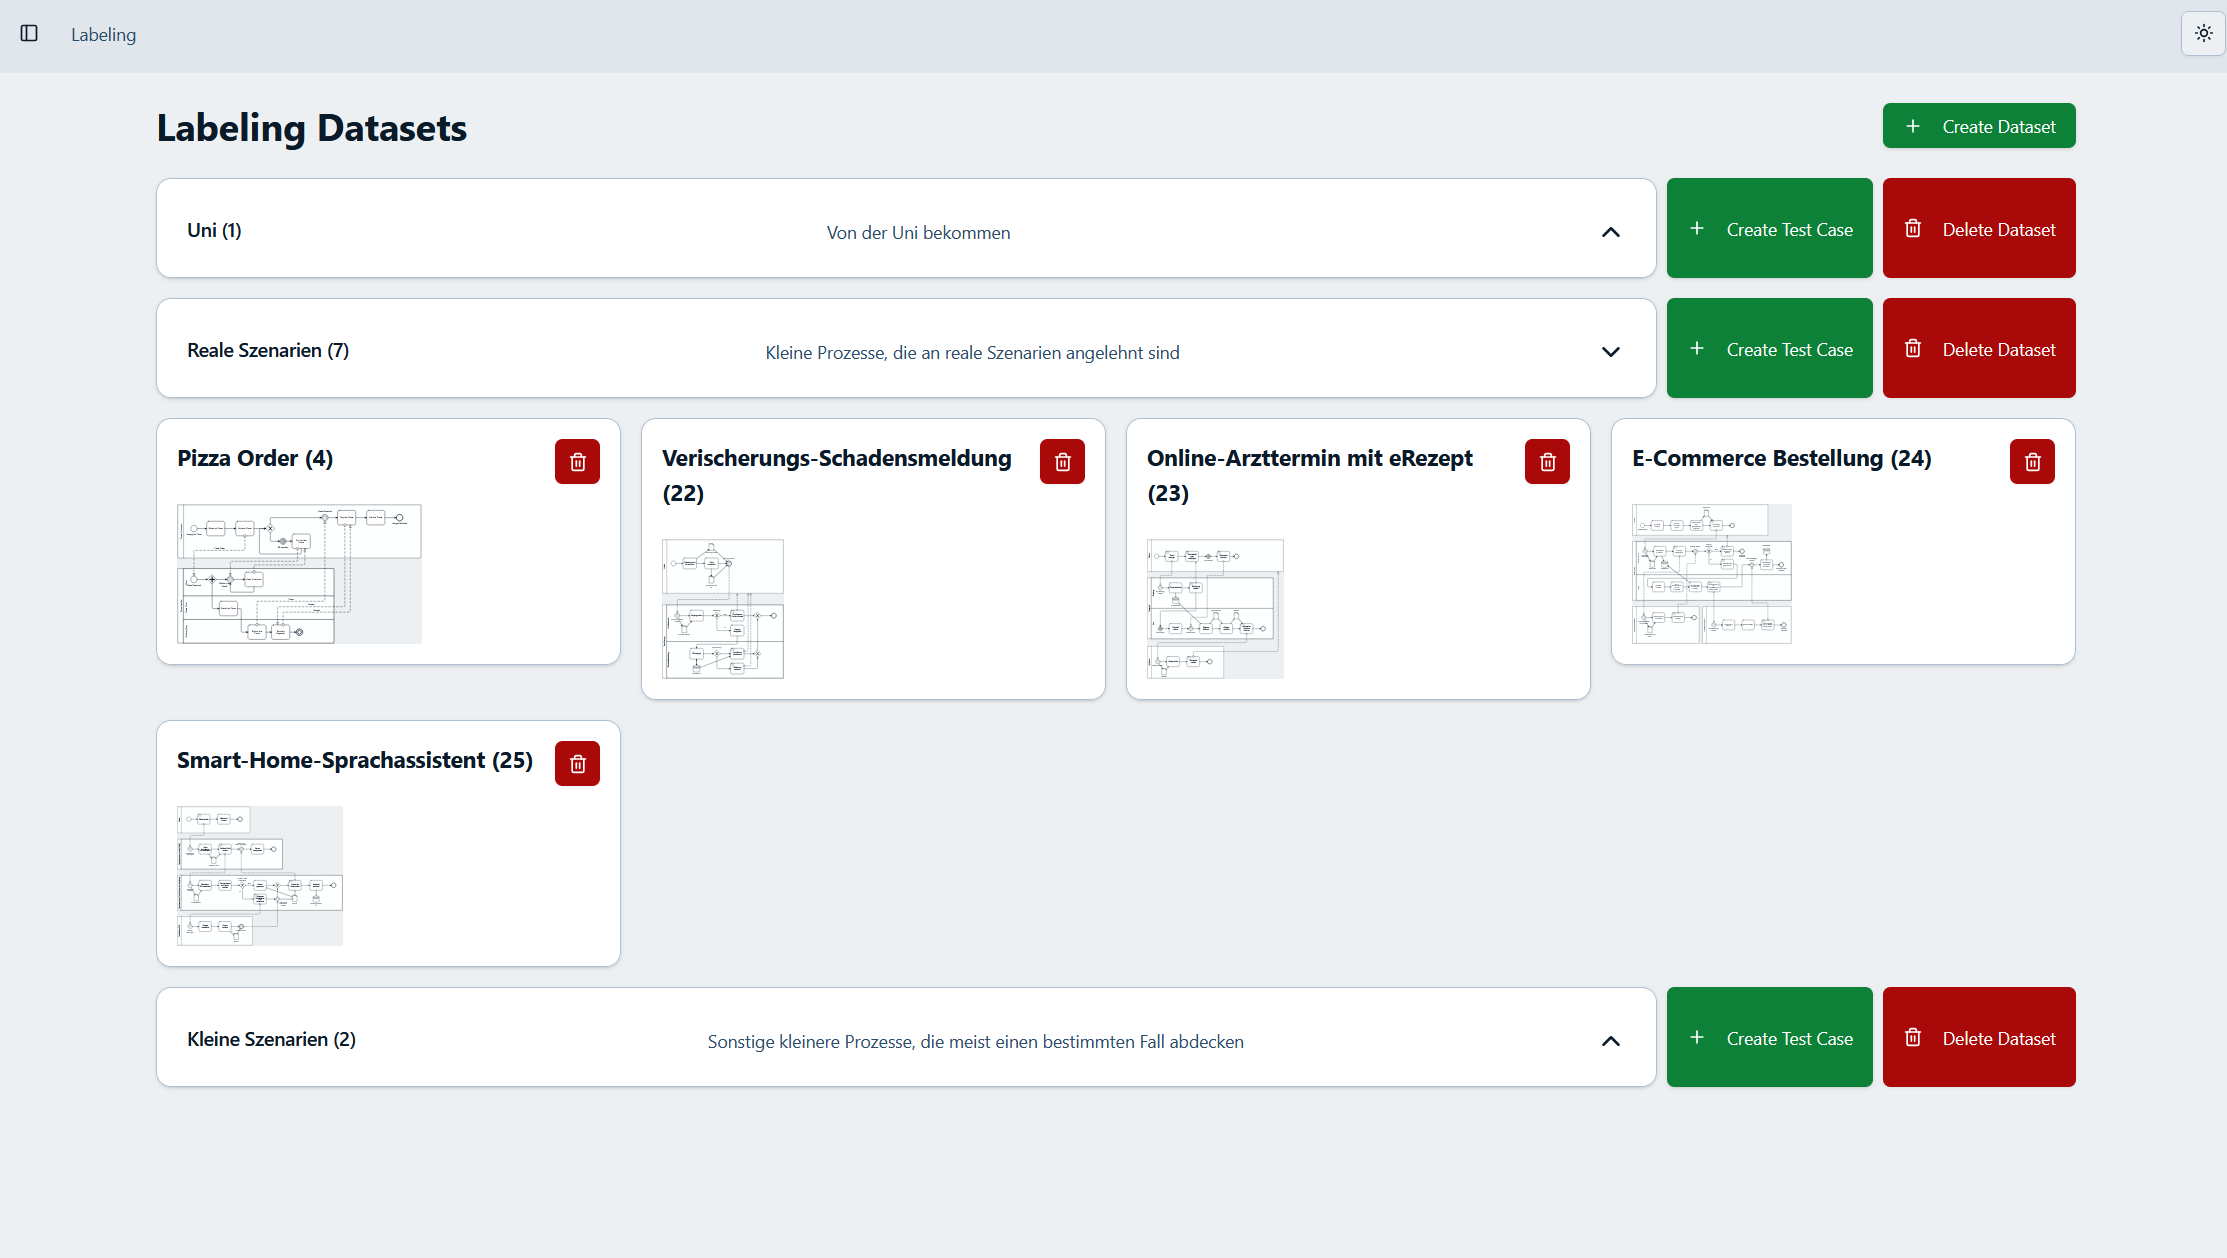
\includegraphics[width=\textwidth]{images/labeling/labeling-datasets}
    \caption{Übersicht der Datensätze im Labeling-Tool.}
    \label{fig:labeling-datasets}
\end{figure}
\section{Quellen und Eigenschaften der Datensätze}\label{sec:quellen-und-eigenschaften-der-datensatze}

Für die Evaluation wurden drei Gruppen von \ac{BPMN}-Datensätzen eingesetzt:

\begin{enumerate}
    \item Prozesse, die von der Universität Ulm bereitgestellt wurden (z.B.\ Lehrbeispiele aus Übungsaufgaben).
    \item Mittelgroße Praxisbeispiele aus verschiedenen Domänen. Diese Prozesse beinhalten Elemente wie Pools, Lanes, Datenobjekte und Gateways.
    \item Kleine, reduzierte Testfälle mit maximal fünf Aktivitäten und wenigen weiteren Elementen (z.\,B. einfacher Sequenzfluss ohne Pools).
\end{enumerate}

Die Praxisbeispiele (Gruppe\,2) decken typische \emph{geschäftliche Domänen} ab, darunter kundenorientierte Service- und Bestellprozesse (E-Commerce), fachliche Abläufe im Versicherungs- und Gesundheitswesen sowie technische Smart-Home/IoT-Kontexte. Die universitären Beispiele (Gruppe~1) stammen aus lehrnahen Übungsaufgaben und stellen Domänen wie wie Finanzen, Logistik und HR dar. Die kleinen Testfälle (Gruppe\,3) sind bewusst minimal gehalten, um Randfälle und unterschiedliche Modellkomplexitäten abzudecken.

Diese bewusst heterogene Auswahl über Domänen, Sprachen und Komplexitätsstufen erhöht die Aussagekraft der Evaluation. In der Literatur wird betont, dass eine erhöhte Datensatzvielfalt die Robustheit der Bewertung steigert und einseitige Ergebnisse vermeidet \cite{blake2025datasetdiversity}. Tabelle \ref{tab:datensaetze-eckdaten} zeigt die Eckdaten der Datensätze.

\begin{table}[htbp]
    \centering
    \begin{threeparttable}
    \caption{Eckdaten der verwendeten Datensätze}
    \label{tab:datensaetze-eckdaten}
    \begin{tabular}{l r r r}
        \toprule
        & Uni-Prozesse & Reale Szenarien & Kleine Testfälle \\
        \midrule
        Testfälle Gesamt                  & 5  & 5 & 14 \\
        Testfälle (DE)                    & 0 & 3 & 15 \\
        Testfälle (EN)                    & 5 & 2 & 0 \\
        Ø Aktivitäten $\pm$ SD\tnote{1}   & 13,4 $\pm$ 2,6 & 11,6 $\pm$ 4,2 & 3,9 $\pm$ 1,4 \\
        Ø Aktivitäten (kritisch) $\pm$ SD & 8,6 $\pm$ 3,6 & 6,6 $\pm$ 1,9 & 2,1 $\pm$ 1,5 \\
        Ø Datenobjekte $\pm$ SD           & 1,4 $\pm$ 1,9 & 3,6 $\pm$ 2,1 & 0,4 $\pm$ 0,7 \\
        Ø Datenassoziationen $\pm$ SD     & 2,4 $\pm$ 3,3 & 7 $\pm$ 4 & 0,7 $\pm$ 1,2 \\
        Ø Ereignisse $\pm$ SD             & 21 $\pm$ 13,8 & 8,2 $\pm$ 2,8 & 2 $\pm$ 0 \\
        Ø Gateways $\pm$ SD               & 13 $\pm$ 7,6 & 1,8 $\pm$ 1,5 & 0 $\pm$ 0 \\
        Ø Pools $\pm$ SD                  & 3,4 $\pm$ 1,1 & 3 $\pm$ 1 & 0,4 $\pm$ 0,6 \\
        Ø Lanes $\pm$ SD\tnote{2}         & 3 $\pm$ 1 & 4 $\pm$ 0,7 & 0,3 $\pm$ 0,5 \\
        Ø Nachrichtenflüsse $\pm$ SD      & 9,4 $\pm$ 5,3 & 5,2 $\pm$ 0,8 & 0,1 $\pm$ 0,3 \\
        Ø Annotationen $\pm$ SD           & 1 $\pm$ 1,7 & 0 $\pm$ 0 & 0 $\pm$ 0 \\
        \bottomrule
    \end{tabular}
    \begin{tablenotes}
        \item[1] SD = Standardabweichung $s$ der jeweiligen Anzahl pro Testfall.
        \item[2] Blackbox-Pools ohne Lanes wurden nicht mitgezählt, daher kann der Durchschnittswert der Lanes geringer ausfallen als der, der Pools.
    \end{tablenotes}
    \end{threeparttable}
\end{table}
\section{Labeling-Guide}\label{sec:labeling-guide}

Die Aktivitäten in den Testfällen sollen mit dem Label \enquote{kritisch} versehen werden, wenn sie potenziell personenbezogene Daten verarbeiten und somit im Sinne der \ac{DSGVO} relevant sein könnten. Die wichtigsten Begriffe der \ac{DSGVO} wurden bereits in Abschnitt \ref{sec:dsgvo} definiert.

Beim Labeln einer Aktivität können Grenzfälle auftreten, insbesondere wenn kein Datenobjekt vorhanden ist, der Name einer Aktivität aber auf Datenverarbeitung hinweist, wie z.\,B. \enquote{Verträge archivieren}. Dabei kann es sich sowohl um personenbezogene Verträge, wie Arbeitsverträge, als auch um rein geschäftliche Verträge zwischen Unternehmen handeln. In einem solchen Fall wird zuerst geschaut, ob der Kontext der Aktivität Hinweise auf personenbezogene Daten gibt (z.\,B. Pool/Lane oder andere Aktivitäten im Prozess). Wenn keine eindeutigen Hinweise vorliegen, wird die Aktivität als unkritisch gelabelt. Wenn jedoch der Kontext auf die Verarbeitung personenbezogener Daten hinweist (z.\,B. ein Prozessname wie \enquote{Mitarbeiterverwaltung} oder vorherigere Aktivitäten wie \enquote{Mitarbeiterdaten erfassen}), wird die Aktivität als kritisch gelabelt. Im Zweifel wird die Aktivität als kritisch gelabelt, um eine höhere Sensitivität zu gewährleisten.

Tabelle \ref{tab:labeling-examples} listet beispielhaft einige Aktivitäten mit ihrer Klassifikation und einer Begründung auf.

\begin{table}[htbp]
    \centering
    \caption{Beispielhafte Aktivitäten und Label}
    \begin{tabularx}{\textwidth}{p{0.4\textwidth} c p{0.4\textwidth}}
        \toprule
        Aktivität & Kritisch? & Kommentar \\
        \midrule
        Lieferadresse eingeben & Ja & Name, Anschrift des Kunden werden aufgenommen. \\
        Rückfrage an Kunden senden & Ja & Kontaktinformationen werden verwendet. \\
        Fall anlegen & Ja & Aktivität befindet sich im Kundenservice-Kontext, personenbezogene Daten wahrscheinlich. \\
        Sprache zu Text verarbeiten & Ja & Im Kontext eines Sprachassistenten werden biometrische Daten des nutzers verarbeitet. \\
        Produkt versenden & Nein^* & Logistik und Sachvorgänge sind nicht per se Datenschutzkritisch, solange keine neue Datenverarbeitung, wie ein Labeldruck stattfindet. \\
        Systemprotokoll auslesen & Ja & Im Kontext einer technischen Wartung können personenbezogene Daten (z.\,B. Nutzer-\texttt{ids}) enthalten sein. \\
        Logdaten archivieren (anonym) & Nein & Keine personenbezogenen Daten enthalten. \\
        Gerät kalibrieren & Nein & Im Kontext einer technischen Wartung werden keine personenbezogenen Daten verarbeitet. \\
        \bottomrule
    \end{tabularx}
    \label{tab:labeling-examples}
\end{table}